
\documentclass{standalone} %\documentclass[conference,10pt]{IEEEtran}
% \usepackage{amsmath}
%\ifCLASSINFOpdf
  % \usepackage[pdftex]{graphicx}
  % declare the path(s) where your graphic files are
  % \graphicspath{{../pdf/}{../jpeg/}}
  % and their extensions so you won't have to specify these with
  % every instance of \includegraphics
  % \DeclareGraphicsExtensions{.pdf,.jpeg,.png}
%v\else
  % or other class option (dvipsone, dvipdf, if not using dvips). graphicx
  % will default to the driver specified in the system graphics.cfg if no
  % driver is specified.
  % \usepackage[dvips]{graphicx}
  % declare the path(s) where your graphic files are
  % \graphicspath{{../eps/}}
  % and their extensions so you won't have to specify these with
  % every instance of \includegraphics
  % \DeclareGraphicsExtensions{.eps}
%\fi

\usepackage[caption=false,font=footnotesize]{subfig} %ERIC Added
\usepackage{float}	%ERIC added

\usepackage{color}	% required for `\textcolor' (yatex added)
%%%ERIC REMOVED: \usepackage[dvipdfmx]{graphicx}
% \usepackage[dvips]{graphicx} %-->> for pdftex use: \usepackage[pdftex]{graphicx}

\usepackage{xcolor, tikz, pgfplots, ifthen}
\usepackage[american,cuteinductors,smartlabels]{circuitikz}
\pgfplotsset{compat=newest}
\usetikzlibrary{intersections,patterns}
\usetikzlibrary{calc}
\usetikzlibrary{backgrounds,positioning}
%\usetikzlibrary{arrows}
\newlength\figureheight
\newlength\figurewidth 

\definecolor{sthlmRed}{RGB}{196,0,100} % HEX #fedeed
\definecolor{sthlmBlue}{RGB}{0,110,191} % HEX #006ebf
\definecolor{sthlmGreen}{RGB}{0,134,127} % #00867f
\newcommand{\al}[1]{\textcolor{sthlmRed}{#1}}

\begin{document}

\centering
	
	%\input{DPNV_Phasors.tex}	
	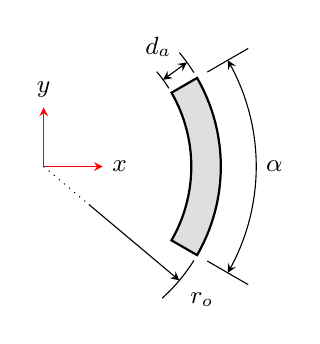
\begin{tikzpicture}[font=\small, >=stealth,scale=1.5]
	%\draw ([shift=(start_coord)] center_x, center_y) arc (start_angle:end_angle:radius);
	\draw[red,<->] (0,.5) node[above] [black]{$y$}[red] -- (0,0)
			-- ++ (.5,0) node[right] [black]{$x$};
	
	\draw[thick,fill=gray!25!white]([shift=(-30:1.5)] 0, 0) arc (-30:30:1.5) 
		-- (30:1.25) 
		arc (30:-30:1.25)
		-- (-30:1.5) -- cycle;
	
	%dimensions
		%arc span
		\draw[] (30:1.6) -- (30:2);
		\draw[] (-30:1.6) -- (-30:2);
		\draw[<->]([shift=(-30:1.8)] 0, 0) arc (-30:30:1.8) node[black, pos=0.5, right] {$\alpha$};

		%outer radius
		\draw[dotted] (0:0) -- (-40:.5); 
		\draw[->] (-40:.5) -- (-40:1.5) node [black, pos=1.25]{$r_o$};
		\draw[]([shift=(-32:1.5)] 0, 0) arc (-32:-48:1.5);
		
		%thickness
		\draw[<->] (36:1.25) -- (36:1.5) node [black, pos=.75,above left]{$d_a$};
		\draw[]([shift=(32:1.5)] 0, 0) arc (32:40:1.5);
		\draw[]([shift=(32:1.25)] 0, 0) arc (32:40:1.25);
	
	\end{tikzpicture}

\end{document}
